\chapter{Interpretability in IR} % Main chapter title

\label{Chapter5} % Change X to a consecutive number; for referencing this chapter elsewhere, use \ref{ChapterX}

\lhead{Chapter 5. \emph{Interpretability in IR}} % Change X to a consecutive number; this is for the header on each page - perhaps a shortened title

In this chapter, we will initially describe how the interpretability approaches detailed in chapter~\ref{Chapter3}--LIME (section~\ref{sec:lime_approach}) and DeepSHAP (section~\ref{sec:deepshap_approach}) are applied for \textit{ad-hoc} text retrieval and ranking in the context of complex neural ranking models. 

In this work, we are interested in how DeepSHAP can be adapted to explain the output of neural retrieval models (NRM). In particular, what is a good ``\textit{reference}'' input in the context of IR? In computer vision, a plain black image is a good reference input to understand the decisions of a image classifier. So we developed various reference input document construction methods as described in the section~\ref{sec:deepshap_ir} for 3 different neural rankers (DRMM, MatchPyramid, PACRR-DRMM). We would also like to investigate if DeepSHAP's explanations are highly sensitive or robust to the different reference input distributions that were constructed. Also, do these reference input distributions perform differently depending on the neural ranking model. Additionally, we compare the explanations produced by DeepSHAP to that of LIME (model-agnostic) detailed in section~\ref{sec:lime_ir}. We ponder on the question, if both these approaches produce different or similar explanations, as they both give \textit{local} explanations. 

In order to understand the various questions raised above, we describe the experimental setup in section~\ref{sec:lime_shap_exp_setup}. The results of the various experiments are discussed in detail in section~\ref{sec:lime_shap_results}.

%-----------------------------------------------------
%	SECTION 1
%-----------------------------------------------------
\section{LIME for IR}\label{sec:lime_ir}

\begin{figure}[]
  \centering
  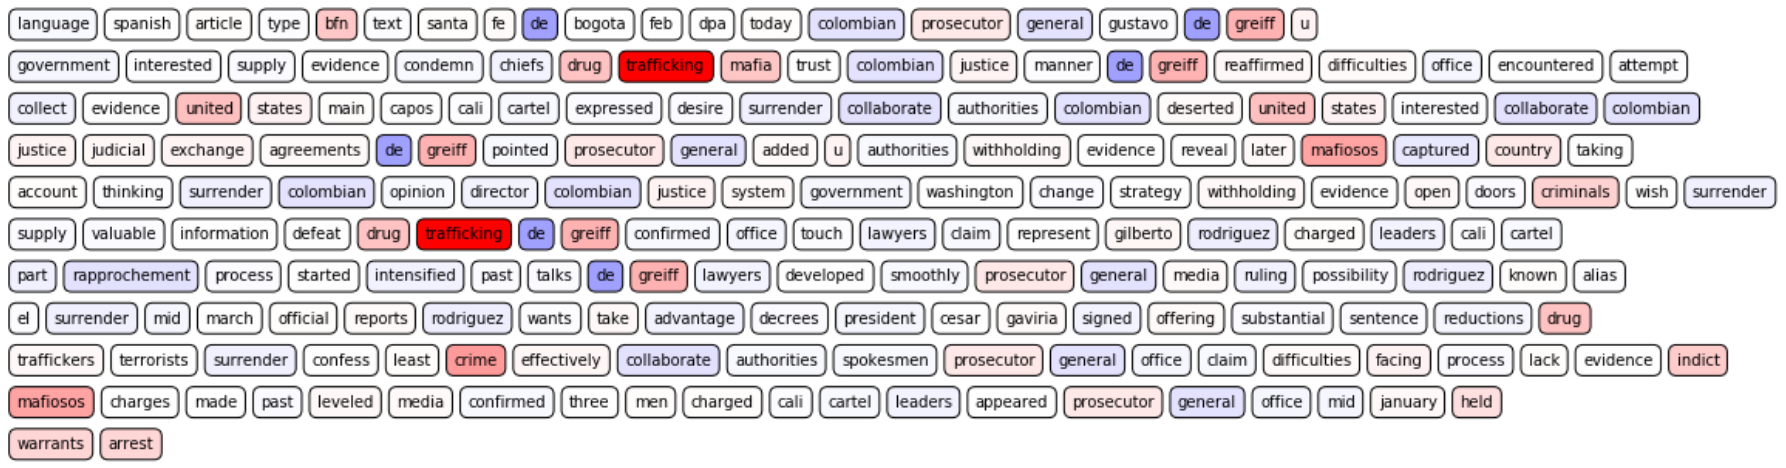
\includegraphics[width=\textwidth]{Figures/q301_FBIS3-10082_lime_drmm.png}
  \caption[Heatmap visualization of document using LIME relevance weights for DRMM.]{Heatmap visualization over the words in the doc `\textsf{FBIS3-10082}' for the query `\textsf{international organized crime}' using the output of LIME for the DRMM ranking model. \textit{Words highlighted in `red' indicate `relevance' and those in `blue' for the `irrelevant' class.}}
  \label{fig:drmm_lime_heatmap}
\end{figure}

The LIME~\citep{Ribeiro16} approach is designed mainly to explain the output of classifiers, whereas we would like to understand \textit{why} a particular document returned from a neural retrieval model is relevant to a query. Recently, there has been work~\citep{Singh19} which adapted LIME to show how ranking can be cast as a classification problem where the neural retrieval model predicts a class distribution (\textit{relevant} or \textit{irrelevant}) for a given query-document pair. We discuss their {\it score-based} approach that we implemented here, consider a query {\it q} and the list of {\it top-k} documents $D^{k}_{q}$ returned from the neural retrieval model $\mathcal{R}$ (point-wise ranker) obtained by scoring each document from a set of candidate documents retrieved from the index (BM25) and sorting. To explain a document $d$ from $D^{k}_{q}$, LIME trains an explanation model $\mathcal{M}_{d}$ on the perturbed documents $d'$. To model it into a classification problem they consider a random variable $\mathcal{X}$ to indicate the possible classes - \textit{relevant} and \textit{irrelevant}. Below is the formula used to compute $P(\mathcal{X} = relevant|q,d',\mathcal{R})$ using the {\it score-based} approach,
\begin{equation}
    1 - \frac{\mathcal{R}(q,d_{1}) - \mathcal{R}(q,d')}{\mathcal{R}(q,d_{1})}
\end{equation}
where $d_{1} \in D^{k}_{q}$ is the top-ranked document in the list, if $\mathcal{R}(q,d') \geq \mathcal{R}(q,d_{1})$ then $P(\mathcal{X}=relevant) = 1$. Note that $P(\mathcal{X} = irrelevant|q,d',\mathcal{R}) = 1 - P(\mathcal{X} = relevant|q,d',\mathcal{R})$.

\textbf{Explanation Model} In this approach the interpretable feature space is the set of words and since the explanation model $\mathcal{M}_{d}$ is a linear ridge regression model, the sign and magnitude of the coefficients of $\mathcal{M}_{d}$ indicate which words in $d$ are strong indicators of relevance and could be used as visual explanations such as heatmaps over the input words as shown in Figure~\ref{fig:drmm_lime_heatmap}.


\section{DeepSHAP for IR}\label{sec:deepshap_ir}

In the context of IR, DeepSHAP can be used to explain \textit{why} a document is relevant to query (according to a given neural retrieval model) by computing the shapley values for words in the document. The words with high shapley values indicate that they are important towards this prediction of relevance. However, to accurately compute the shapley values using DeepSHAP--a reference input is needed. What makes a good \textit{background} image in the context of IR? 

Unlike classification tasks, in ranking we have at least 2 inputs which are in most cases the query and document tokens. In this work, we fix the reference input for the query to be same as that of the query-document instance to be explained and experiment with various reference inputs for the document. The intuition behind doing so is to gain an average reference output in the locality of the query. 

The various document reference inputs that we considered in our experiments are:
\begin{description}
    \item[OOV] The reference document consists of `OOV' tokens. For, DRMM and MatchPyramid models the embedding vector for `OOV' comprises of all-zeros which is similar to the background image used for MNIST. But for PACRR-DRMM the `OOV' embedding vector is the average of all the embedding vectors in the vocabulary. 
    \item[IDF {\it lowest}] The reference document is constructed by sampling words with low IDF scores. These words are generally stop-words or words that are similar to stop-words so they should, in general, be irrelevant to the query. 
    \item[QL {\it lowest}] The reference document comprises of sampled words with low {\it query-likelihood} scores that are derived from a language model of the {\it top-1000} documents. As this would have words that are irrelevant to the query, SHAP should be able to pick more relevant terms from the document to be explained.
    \item[COLLECTION {\it rand doc}] The reference document is randomly sampled from the rest of the collection minus the {\it top-1000} documents retrieved for the query.
    \item[TOPK LIST {\it rand doc from bottom}] The reference document is randomly sampled from the bottom of the {\it top-1000} documents retrieved.
\end{description}

These variants were designed based on the intuition that the reference input document would comprise of words that are irrelevant to the query and thus DeepSHAP should be able to pick the most important terms from the input document that explain relevance to the query.

\section{Experimental Setup}
\label{sec:lime_shap_exp_setup}
In our experiments, we aim to answer the following research questions:

\begin{itemize}
    \item \textbf{RQ1} Are DeepSHAP explanations sensitive to the type of reference input in the case of NRMs?
    \item \textbf{RQ2} Can we determine which reference input produces the most accurate local explanation?
    \item \textbf{RQ3} Does modeling the reference distribution for query input also affect the DeepSHAP explanations?
\end{itemize}

To this end, we describe the experimental setup we used to address these questions. The 3 neural ranking models that we considered are--DRMM, MatchPyramid (MP-COS), and PACRR-DRMM. All the models were trained using the setup as described in chapter~\ref{Chapter4}. Once trained all the models were deployed using the Flask web framework as detailed in section~\ref{sec:deploy_nrm}.

To conduct the experiments, we used the Robust04 test collection from TREC. We used Lucene to index and retrieve documents. We chose to study explanations for the distinguished set of hard topics\footnote{\url{https://trec.nist.gov/data/robust/04.guidelines.html}} (50) from the TREC Robust Track 2004 (model retrieval effectiveness highlighted in Tab~\ref{tab:robust04_difficult_rank_measures}). We generate the explanations from LIME and SHAP for the top-3 documents retrieved for each query and use only these for our quantitative experiments.

\begin{table}[h]
\centering
\begin{tabular}{lcccccc} 
 \toprule
 & MAP & MRR & P@10 & P@20 & NDCG@10 & NDCG@20\\
 \midrule
 BM25 & 0.0890 & 0.4786 & 0.2280 & 0.2030 & 0.2462 & 0.2289\\
 DRMM & 0.1202 & 0.5444 & 0.2900 & 0.2430 & 0.3103 & 0.2781\\
 MatchPyramid & 0.0855 & 0.4466 & 0.2420 & 0.2140 & 0.2512 & 0.2340\\
 PACRR-DRMM & 0.1036 & 0.4704 & 0.2720 & 0.2310 & 0.2780 & 0.2545\\
 \bottomrule
\end{tabular}
\caption{Overview of models retrieval effectiveness for the ROBUST04 hard queries}
\label{tab:robust04_difficult_rank_measures}
\end{table}

\textbf{Evaluating explanations} Since no ground truth explanations are available for a neural model, we use LIME based explanations as a proxy. Although LIME is model agnostic, we found that it can accurately model relevance for a given query document pair using a simple linear model over words. Table~\ref{tab:lime_model_performances} shows this observation, where the number of perturbed samples for every query-document pair is divided into train (90\%) and test (10\%) splits. To produce the explanations from LIME we used the implementation found in \footnote{\url{https://github.com/marcotcr/lime}} along with the score-based modification described in section~\ref{sec:lime_ir}. The primary parameters for training a LIME explanation model are the number of perturbed samples to be considered and the number of words for the explanation. The number of perturbed samples is set to 5000 and the number of words is varied based on the experiment. We used the DeepSHAP implementation provided here~\footnote{\url{https://github.com/slundberg/shap}}. Note that we ignore the polarity of the explanation terms provided by both methods in our comparison since the semantics behind the polarities in LIME and DeepSHAP are different. We are more interested in the terms chosen as the explanations in both cases.

For the SHAP explanations we used the methods as described in Section \ref{sec:deepshap_ir}. Since the model inputs for MatchPyramid and PACRR-DRMM directly accept document tokens it is a one-to-one mapping from the tokens to the corresponding SHAP value. But for DRMM, the model inputs are query-document histograms and thus we obtain SHAP values for these histogram buckets. So in order to map these SHAP values back to the document tokens we store a mapping from the tokens to their respective histogram buckets.

\begin{table}
\centering
\begin{tabular}{lcccc} 
 \toprule
 &\multicolumn{4}{c}{Linear Regression (Ridge)}\\
 NRM & TRAIN MSE & TEST MSE & TRAIN ACC & TEST ACC\\
 \midrule
 DRMM & 0.00631 & 0.00633 & 0.92662 & 0.92654\\
 MatchPyramid & 0.01827 & 0.01839 & 0.90367 & 0.90387\\
 PACRR-DRMM & 0.00165 & 0.00160 & 0.98857 & 0.98980\\
\bottomrule
\end{tabular}
\footnotesize
\caption[Evaluation of LIME's linear model performance metrics across various NRMs.]{Comparison of mean squared error (MSE) and accuracy (ACC) of LIME's linear model across various NRMs. Low MSE and high accuracy shows that it is able to fit and generalize in the query-document locality.}
\label{tab:lime_model_performances}
\end{table}


\section{Results and Discussion}
\label{sec:lime_shap_results}

\subsection{RQ1. Effect of reference input document} \label{sec:interpretability_rq1}

The top row in Figure~\ref{fig:shap_confusion_matrices} illustrates the overlap in terms of jaccard similarity between the explanation terms produced when varying the reference input. Immediately we observe that the overlap between explanations produced is low; below 50\% in most cases and consistently across all NRMs. Each reference input method has its own distinct semantics and this is reflected by the low overlap scores. This is also shown by the high Jensen-Shannon divergence scores (2nd row in Fig.~\ref{fig:shap_confusion_matrices}) between the probability distributions of the term coefficients returned by each reference input method. We also find that there is no consistent trend across NRMs. For MatchPyramid, \textsf{OOV} and \textsf{QL} have highest overlap whereas for PACRR-DRMM its \textsf{OOV} and \textsf{COL} that have highest overlap even though both models have the same input representation and parts of the model architecture are similar (convolutional and max-pooling layers). Table~\ref{tab:drmm_qualitative_example} shows explanations for DRMM across all variants. Once again we see how the explanations can differ significantly if we are not careful in selecting the reference input. For IR, finding the background image seems to be a much harder question. 

Our results show how explanations are highly sensitive to the reference input for NRMs chosen in our experiments. This is also indication that a single reference input method may not be the best for every NRM. 

\begin{figure}
  \centering
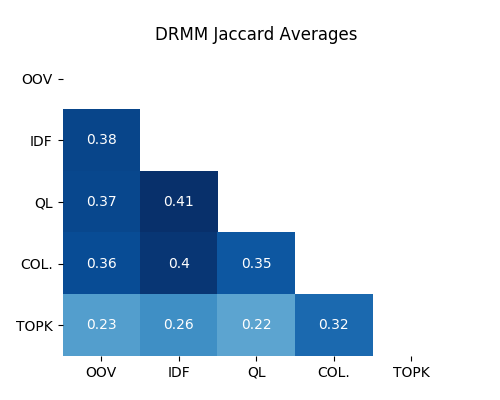
\includegraphics[width=.33\linewidth]{Figures/drmm_jaccard.png}\hfill
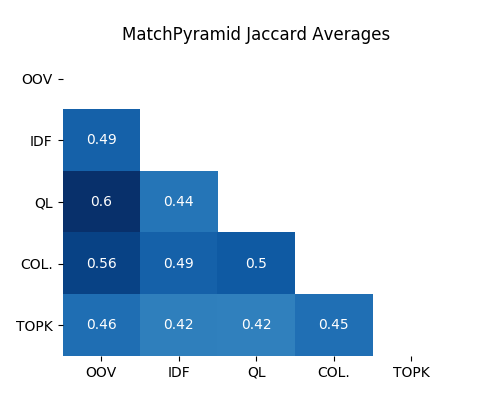
\includegraphics[width=.33\linewidth]{Figures/mp_cos_jaccard.png}\hfill
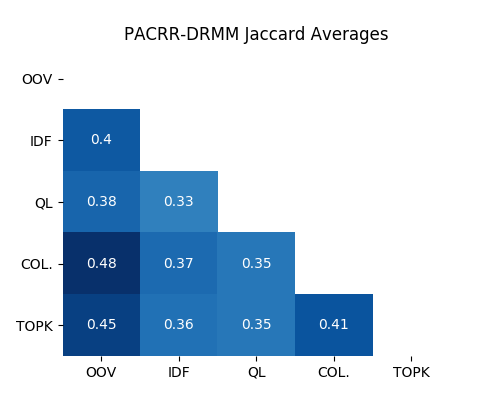
\includegraphics[width=.33\linewidth]{Figures/pacrr_drmm_jaccard.png}
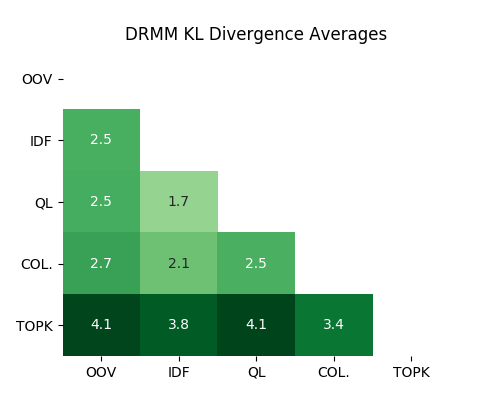
\includegraphics[width=.33\linewidth]{Figures/drmm_kl_div.png}\hfill
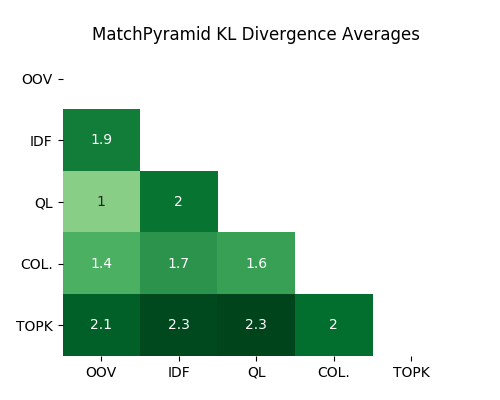
\includegraphics[width=.33\linewidth]{Figures/mp_cos_kl_div.png}\hfill
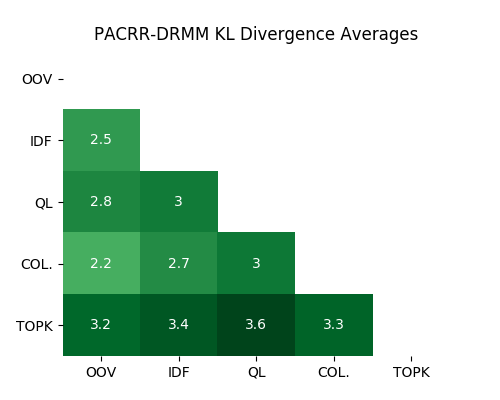
\includegraphics[width=.33\linewidth]{Figures/pacrr_drmm_kl_div.png}
  \caption[Confusion matrices of DeepSHAP background documents comparing Jaccard similarities and Jensen-Shannon divergence.]{Confusion matrices of various DeepSHAP background document methods comparing the overlap in terms of both Jaccard similarities and Jensen-Shannon divergence.}
  \label{fig:shap_confusion_matrices}
\end{figure}


\begin{table}[h]
    \centering
    \begin{tabular}{cccccc}
        \toprule
        LIME & OOV & IDF & QL & COL. & TOPK\\
        \midrule
cult & cult & cult & cult & cult & cult \\
style & followers & style & style & black & {\bf numbers} \\
followers & black & followers & elite & fraternities & {\bf english} \\
elite & fraternities & {\bf suspects} & saloon & degenerate & {\bf college} \\
saloon & degenerate & {\bf belong} & {\bf final} & sons & {\bf university} \\
{\bf student} & sons & {\bf reappearing} & march & followers & {\bf fallouts} \\
home & {\bf academic} & household & {\bf friday} & style & {\bf buccaneers} \\
{\bf members} & {\bf american} & black & september & home & {\bf feudings} \\
march & {\bf tried} & fraternities & {\bf arms} & household & {\bf activists} \\
september & household & degenerate & {\bf closed} & {\bf avoid} & {\bf troubles} \\
        \bottomrule
    \end{tabular}
    \caption[Comparison of explanations from LIME and various DeepSHAP methods for an example document with DRMM.]{An example of words selected by LIME and various DeepSHAP methods with the \textsf{DRMM} model for the query {\bf `cult lifestyles'} and document {\bf `FBIS3-843'} which talks about clashes between cult members and student union's activists at a university in Nigeria. {\it Words unique to a particular explanation method are highlighted in bold}.}
    \label{tab:drmm_qualitative_example}
\end{table}

\subsection{RQ2. Accuracy of reference input methods}\label{sec:interpretability_rq2}

\begin{table}
\footnotesize
\centering
\begin{tabular}{lccc} 
 \toprule
 & DRMM & MatchPyramid & PACRR-DRMM \\
 \midrule

%LIME & 1.000 $\pm$ 0.000 & 1.007 $\pm$ 0.084 & 0.999 $\pm$ 0.004\\
%\cmidrule(lr){2-4}

OOV & 1.000 $\pm$ 0.000 & 0.498 $\pm$ 0.087 & 0.125 $\pm$ 0.077\\
% \cmidrule(lr){2-4}

IDF & 0.998 $\pm$ 0.021 & 0.500 $\pm$ 0.087 & 0.196 $\pm$ 0.113\\
% \cmidrule(lr){2-4}

QL std. form. & 0.998 $\pm$ 0.012 & 0.517 $\pm$ 0.083 & 0.205 $\pm$ 0.114\\
% \cmidrule(lr){2-4}

COLLECTION & 0.999 $\pm$ 0.004 & 0.500 $\pm$ 0.087 & 0.164 $\pm$ 0.083\\
% \cmidrule(lr){2-4}

TOPK LIST. & 0.999 $\pm$ 0.006 & 0.518 $\pm$ 0.095 & 0.162 $\pm$ 0.078\\
\bottomrule
 \end{tabular}
 \caption{Comparison of mean and standard deviation of the fraction of terms returned from LIME and DeepSHAP for ROBUST04 hard queries}
\label{tab:queries_diff_mean_std_terms_shap}
\end{table}

To help identify which reference input method is most accurate in explaining a given query-document pair, we compared the LIME explanations for the same against it's corresponding DeepSHAP explanation methods. In general we found that DeepSHAP produces more explanation terms (see Table~\ref{tab:queries_diff_mean_std_terms_shap}) whereas LIME's L1 regularizer constrains the explanations to only the most important terms (10, 20, 30). Additionally, the discrepancy between the explanations can be attributed to LIME being purely \textit{local}, whereas DeepSHAP has some \textit{global} context since it looks at activations for the whole network which may have captured some global patterns. Hence to estimate which reference input surfaces the most `ground truth' explanation terms we only computed recall at top 50 and 100 (by shapley value magnitude) DeepSHAP explanation terms (in Table~\ref{tab:doc_bg_dist_recall}).

\begin{table}[h]
\scalebox{0.6}{
\begin{tabular}{ m{6em}m{2em}m{2em}m{2em}m{2em}m{2em}m{2em}m{2em}m{2em}m{2em}m{2em}m{2em}m{2em}m{2em}m{2em}m{2em}m{2em}m{2em}m{2em}} 
\toprule
 &\multicolumn{6}{c}{DRMM}&\multicolumn{6}{c}{MatchPyramid}&\multicolumn{6}{c}{PACRR-DRMM}\\
 \cmidrule(r){2-7}
 \cmidrule(r){8-13}
 \cmidrule(r){14-19}
 &\multicolumn{2}{c}{top-10} &\multicolumn{2}{c}{top-20}&\multicolumn{2}{c}{top-30} &\multicolumn{2}{c}{top-10}&\multicolumn{2}{c}{top-20}&\multicolumn{2}{c}{top-30}
 &\multicolumn{2}{c}{top-10}&\multicolumn{2}{c}{top-20}&\multicolumn{2}{c}{top-30}\\
 \cmidrule(r){2-3}
 \cmidrule(r){4-5}
 \cmidrule(r){6-7}
 \cmidrule(r){8-9}
 \cmidrule(r){10-11}
 \cmidrule(r){12-13}
 \cmidrule(r){14-15}
 \cmidrule(r){16-17}
 \cmidrule(r){18-19}
 SHAP \newline variants & recall\newline @50  & recall\newline @100 & recall\newline @50  & recall\newline @100 & recall\newline @50  & recall\newline @100 & recall\newline @50  & recall\newline @100 & recall\newline @50  & recall\newline @100 & recall\newline @50  & recall\newline @100 & recall\newline @50  & recall\newline @100  & recall\newline @50  & recall\newline @100 & recall\newline @50  & recall\newline @100\\
 \midrule

OOV & 0.789 & 0.905 & 0.672 & 0.845 & 0.615 & 0.812 & {\bf 0.793} & {\bf 0.843} & {\bf 0.656} & {\bf 0.726} & {\bf 0.566} & {\bf 0.640} & 0.582 & 0.582 & 0.388 & 0.388 & 0.299 & 0.299\\
% \cmidrule(l){2-19}
\addlinespace[1em]

IDF & 0.830 & 0.917 & 0.723 & 0.871 & 0.658 & 0.841 & 0.795 & 0.832 & 0.653 & 0.711 & 0.565 & 0.633 & 0.633 & 0.633 & 0.446 & 0.446 & 0.362 & 0.362\\
% \cmidrule(l){2-19}
\addlinespace[1em]

QL & {\bf 0.894} & {\bf 0.955} & {\bf 0.754} & {\bf 0.892} & {\bf 0.670} & {\bf 0.856} & 0.765 & 0.821 & 0.638 & 0.711 & 0.556 & 0.636 & {\bf 0.643} & {\bf 0.643} & {\bf 0.462} & {\bf 0.462} & {\bf 0.367} & {\bf 0.367}\\
% \cmidrule(l){2-19}
\addlinespace[1em]

% QL inv. rank \newline \textit{lowest} & 0.897 & 0.958 & 0.752 & 0.892 & 0.666 & 0.854 & 0.790 & 0.838 & 0.654 & 0.720 & 0.566 & 0.638 & 0.627 & 0.627 & 0.448 & 0.448 & 0.362 & 0.362\\
% \hline

% IDF-QL \newline \textit{lowest} & 0.893 & 0.957 & 0.749 & 0.892 & 0.664 & 0.854 & 0.790 & 0.838 & 0.654 & 0.720 & 0.566 & 0.638 & 0.627 & 0.627 & 0.448 & 0.448 & 0.362 & 0.362\\
% \hline

% IDF-QL \newline \textit{rand sample of low scores} & 0.900 & 0.952 & 0.756 & 0.885 & 0.679 & 0.857 & 0.762 & 0.824 & 0.630 & 0.711 & 0.546 & 0.634 & 0.643 & 0.643 & 0.458 & 0.458 & 0.367 & 0.367\\
% \hline

COLLECTION & 0.760 & 0.881 & 0.673 & 0.841 & 0.620 & 0.815 & 0.783 & 0.824 & 0.639 & 0.709 & 0.552 & 0.630 & 0.621 & 0.621 & 0.429 & 0.429 & 0.343 & 0.343\\
% \cmidrule(l){2-19}
\addlinespace[1em]

TOPK LIST. & 0.639 & 0.821 & 0.606 & 0.794 & 0.578 & 0.788 & 0.759 & 0.811 & 0.624 & 0.702 & 0.545 & 0.627 & 0.625 & 0.625 & 0.425 & 0.425 & 0.340 & 0.340\\
\bottomrule

 \end{tabular}}
 \caption[Comparison of recall measures at top-k terms from DeepSHAP against ground-truth terms from LIME.]{Comparison of recall measures at \textit{top-k} (50, 100) terms from DeepSHAP against the \textit{top-k} (10, 20, 30) ground-truth terms from LIME for ROBUST04 hard queries}
\label{tab:doc_bg_dist_recall}
\end{table}

The first interesting insight is that some NRMs are easier to explain whereas others are more difficult. PACRR-DRMM consistently has a recall less than $0.7$ whereas the DeepSHAP explanations of DRMM effectively capture almost all of the LIME explanation terms. When comparing reference input variants within each NRM we find that there is no consistent winner. For DRMM, QL is the best which indicates that sampling terms which are relatively generic for this query in particular is a better `background image' than sampling generic words from the collection (IDF). 

In the case of MatchPyramid, TOPK LIST is the worst performing but it is more difficult to distinguish between the approaches here. The best approach surprisingly is OOV. This can be attributed to how MatchPyramid treats OOV terms. The OOV token is represented by an all-zeros embedding vector that is used for padding the input interaction matrix whereas in DRMM, OOV tokens are filtered out. These preprocessing considerations prove to be crucial when determining the right input reference. Moving on to PACRR-DRMM, we once again find that QL is the best method even though DeepSHAP struggles to find all the LIME terms. It struggles to find more LIME terms because the number of explanation terms returned from DeepSHAP for PACRR-DRMM is only about a small fraction (0.2) of the document. We have left the investigation of why the number of explanation terms returned by DeepSHAP varies based on different NRMs for future work. In Table~\ref{tab:doc_bg_dist_recall_no_q_terms}, we show that we get similar insights as discussed above even if we filter out the query terms from the explanation terms returned from both LIME and SHAP.

\begin{table}[h]
\scalebox{0.6}{
\begin{tabular}{ m{6em}m{2em}m{2em}m{2em}m{2em}m{2em}m{2em}m{2em}m{2em}m{2em}m{2em}m{2em}m{2em}m{2em}m{2em}m{2em}m{2em}m{2em}m{2em} } 
\toprule
 &\multicolumn{6}{c}{DRMM}&\multicolumn{6}{c}{MatchPyramid}&\multicolumn{6}{c}{PACRR-DRMM}\\
 \cmidrule(r){2-7}
 \cmidrule(r){8-13}
 \cmidrule(r){14-19}
 &\multicolumn{2}{c}{top-10} &\multicolumn{2}{c}{top-20}&\multicolumn{2}{c}{top-30} &\multicolumn{2}{c}{top-10}&\multicolumn{2}{c}{top-20}&\multicolumn{2}{c}{top-30}
 &\multicolumn{2}{c}{top-10}&\multicolumn{2}{c}{top-20}&\multicolumn{2}{c}{top-30}\\
 \cmidrule(r){2-3}
 \cmidrule(r){4-5}
 \cmidrule(r){6-7}
 \cmidrule(r){8-9}
 \cmidrule(r){10-11}
 \cmidrule(r){12-13}
 \cmidrule(r){14-15}
 \cmidrule(r){16-17}
 \cmidrule(r){18-19}
 SHAP \newline variants & recall\newline @50  & recall\newline @100 & recall\newline @50  & recall\newline @100 & recall\newline @50  & recall\newline @100 & recall\newline @50  & recall\newline @100 & recall\newline @50  & recall\newline @100 & recall\newline @50  & recall\newline @100 & recall\newline @50  & recall\newline @100  & recall\newline @50  & recall\newline @100 & recall\newline @50  & recall\newline @100\\
 \midrule

% OOV \newline w padding & 0.762 & 0.888 & 0.654 & 0.836 & 0.603 & 0.805 & 0.762 & 0.813 & 0.633 & 0.703 & 0.548 & 0.620 & 0.475 & 0.475 & 0.316 & 0.316 & 0.248 & 0.248\\
% \hline

OOV & 0.762 & 0.888 & 0.654 & 0.836 & 0.603 & 0.805 & \textbf{0.762} & \textbf{0.812} & \textbf{0.633} & \textbf{0.702} & \textbf{0.548} & \textbf{0.619} & 0.472 & 0.472 & 0.315 & 0.315 & 0.245 & 0.245\\
\addlinespace[1em]

IDF & 0.796 & 0.902 & 0.702 & 0.863 & 0.645 & 0.836 & 0.759 & 0.800 & 0.628 & 0.685 & 0.545 & 0.612 & 0.538 & 0.538 & 0.380 & 0.380 & 0.314 & 0.314\\
\addlinespace[1em]

QL std. form. & \textbf{0.874} & \textbf{0.945} & \textbf{0.737} & \textbf{0.884} & \textbf{0.657} & \textbf{0.851} & 0.719 & 0.782 & 0.609 & 0.684 & 0.536 & 0.614 & \textbf{0.552} & \textbf{0.552} & \textbf{0.399} & \textbf{0.399} & \textbf{0.319} & \textbf{0.319}\\
\addlinespace[1em]

% QL inv. rank \newline \textit{lowest} & 0.878 & 0.951 & 0.738 & 0.885 & 0.654 & 0.849 & 0.751 & 0.805 & 0.626 & 0.694 & 0.546 & 0.617 & 0.529 & 0.529 & 0.383 & 0.383 & 0.314 & 0.314\\
% \hline

% IDF-QL \newline \textit{lowest} & 0.873 & 0.950 & 0.734 & 0.885 & 0.653 & 0.849 & 0.751 & 0.805 & 0.626 & 0.694 & 0.546 & 0.617 & 0.529 & 0.529 & 0.383 & 0.383 & 0.314 & 0.314\\
% \hline

% IDF-QL \newline \textit{rand sample of low scores} & 0.882 & 0.943 & 0.736 & 0.878 & 0.667 & 0.853 & 0.718 & 0.789 & 0.602 & 0.685 & 0.527 & 0.613 & 0.552 & 0.552 & 0.394 & 0.394 & 0.319 & 0.319\\
% \hline

COLLECTION & 0.721 & 0.864 & 0.654 & 0.832 & 0.609 & 0.811 & 0.741 & 0.788 & 0.611 & 0.682 & 0.532 & 0.607 & 0.524 & 0.524 & 0.362 & 0.362 & 0.292 & 0.292\\
\addlinespace[1em]

TOPK LIST. & 0.601 & 0.804 & 0.588 & 0.786 & 0.568 & 0.783 & 0.715 & 0.776 & 0.596 & 0.676 & 0.524 & 0.606 & 0.529 & 0.529 & 0.357 & 0.357 & 0.289 & 0.289\\
\bottomrule

 \end{tabular}}
\caption[Comparison of recall measures at top-k terms from DeepSHAP against ground-truth terms from LIME \textit{not including query terms}.]{Comparison of recall measures at \textit{top-k} (50, 100) terms from DeepSHAP against the \textit{top-k} (10, 20, 30) ground-truth terms from LIME for ROBUST04 hard queries; {\bf From both sets of terms we ignore the query terms}}
\label{tab:doc_bg_dist_recall_no_q_terms}
\end{table}

\subsection{RQ3. Effect of reference query distribution}\label{sec:interpretability_rq3}

In order to understand the effect of using a reference query input distribution along with the different reference document methods, we construct a reference query input by sampling words that have low IDF scores from the collection. We evaluate the DeepSHAP explanations by computing recall at top 50 and 100 with respect to `ground truth' terms (in Table~\ref{tab:q_dist_doc_bg_dist_recall}) as in section~\ref{sec:interpretability_rq2}.

\begin{table}[h]
\scalebox{0.6}{
\begin{tabular}{ m{6em}m{2em}m{2em}m{2em}m{2em}m{2em}m{2em}m{2em}m{2em}m{2em}m{2em}m{2em}m{2em}m{2em}m{2em}m{2em}m{2em}m{2em}m{2em} } 
\toprule
 &\multicolumn{6}{c}{DRMM}&\multicolumn{6}{c}{MatchPyramid}&\multicolumn{6}{c}{PACRR-DRMM}\\
 \cmidrule(r){2-7}
 \cmidrule(r){8-13}
 \cmidrule(r){14-19}
 &\multicolumn{2}{c}{top-10} &\multicolumn{2}{c}{top-20}&\multicolumn{2}{c}{top-30} &\multicolumn{2}{c}{top-10}&\multicolumn{2}{c}{top-20}&\multicolumn{2}{c}{top-30}
 &\multicolumn{2}{c}{top-10}&\multicolumn{2}{c}{top-20}&\multicolumn{2}{c}{top-30}\\
 \cmidrule(r){2-3}
 \cmidrule(r){4-5}
 \cmidrule(r){6-7}
 \cmidrule(r){8-9}
 \cmidrule(r){10-11}
 \cmidrule(r){12-13}
 \cmidrule(r){14-15}
 \cmidrule(r){16-17}
 \cmidrule(r){18-19}
 SHAP \newline variants & recall\newline @50  & recall\newline @100 & recall\newline @50  & recall\newline @100 & recall\newline @50  & recall\newline @100 & recall\newline @50  & recall\newline @100 & recall\newline @50  & recall\newline @100 & recall\newline @50  & recall\newline @100 & recall\newline @50  & recall\newline @100  & recall\newline @50  & recall\newline @100 & recall\newline @50  & recall\newline @100\\
 \midrule
 %\hline\hline

OOV & 0.783 & 0.903 & 0.662 & 0.846 & 0.604 & 0.815 & \textbf{0.789} & \textbf{0.840} & \textbf{0.658} & \textbf{0.730} & \textbf{0.568} & \textbf{0.648} & 0.565 & 0.565 & 0.378 & 0.378 & 0.293 & 0.293\\
\addlinespace[1em]

IDF & 0.885 & 0.948 & 0.751 & 0.897 & 0.664 & 0.858 & 0.754 & 0.813 & 0.627 & 0.712 & 0.553 & 0.643 & 0.646 & 0.646 & 0.459 & 0.459 & 0.372 & 0.372\\
\addlinespace[1em]

QL std. form. & \textbf{0.891} & \textbf{0.954} & \textbf{0.760} & \textbf{0.892} & \textbf{0.676} & \textbf{0.861} & 0.746 & 0.811 & 0.621 & 0.707 & 0.541 & 0.637 & \textbf{0.645} & \textbf{0.645} & \textbf{0.463} & \textbf{0.463} & \textbf{0.380} & \textbf{0.380}\\
\addlinespace[1em]

COLLECTION & 0.824 & 0.901 & 0.699 & 0.850 & 0.640 & 0.821 & 0.756 & 0.815 & 0.626 & 0.707 & 0.545 & 0.633 & 0.613 & 0.613 & 0.422 & 0.422 & 0.335 & 0.335\\
\addlinespace[1em]

TOPK LIST. & 0.818 & 0.907 & 0.698 & 0.857 & 0.634 & 0.827 & 0.746 & 0.803 & 0.619 & 0.695 & 0.540 & 0.622 & 0.610 & 0.610 & 0.418 & 0.418 & 0.334 & 0.334\\

\bottomrule
 \end{tabular}}
\caption[Comparison of recall measures at top-k terms from DeepSHAP using query distribution against ground-truth terms from LIME.]{Comparison of recall measures at \textit{top-k} (50, 100) terms from DeepSHAP using also query distribution sampled from low IDF scores against the \textit{top-k} (10, 20, 30) ground-truth terms from LIME for ROBUST04 hard queries}
\label{tab:q_dist_doc_bg_dist_recall}
\end{table}

Similar to the insights described in section~\ref{sec:interpretability_rq2}, we see that the best performing approaches across each of the models are the same--DRMM (QL), MatchPyramid (OOV) and PACRR-DRMM (QL). Thus, using a reference query input distribution doesn't effect the best performing reference document input variants within each NRM. However, for DRMM we observe that it is now hard to distinguish between various approaches which is different from the insights in Table~\ref{tab:doc_bg_dist_recall}. This could be because of the low activations through the attention network in DRMM from the query reference input due to the use of irrelevant words sampled from IDF. But we don't see such differences in MatchPyramid and PACRR-DRMM, as it was already difficult to distinguish between the approaches when the reference query input was fixed and also these two models don't have an attention network.


% \begin{table}
% \centering
% % \scalebox{0.8}{
% \begin{tabular}{ m{7em}m{2em}m{2em}m{2.8em}m{2em}m{2em}m{2.8em}m{2em}m{2em}m{2.8em}} 
%  \toprule
%  &\multicolumn{3}{c}{DRMM}&\multicolumn{3}{c}{MatchPyramid}&\multicolumn{3}{c}{PACRR-DRMM}\\
%  \cmidrule(lr){2-4}
%  \cmidrule(lr){5-7}
%  \cmidrule(lr){8-10}
%  SHAP variants & recall\newline pos & recall\newline neg & jaccard & recall\newline pos & recall\newline neg & jaccard & recall\newline pos & recall\newline neg & jaccard\\
%  \midrule
% %  OOV \newline w padding & 0.602 & 0.601 & 0.176 & 0.185 & 0.263 & 0.467 & 0.477 & 0.148 & 0.159 & 0.281 & 0.329 & 0.398 & 0.190 & 0.211 & 0.256\\
% % \hline

% OOV & 0.602 & 0.176 & 0.263 & 0.468 & 0.148 & 0.281 & 0.327 & 0.193 & 0.257\\

% IDF \textit{lowest} & 0.633 & 0.126 & 0.283 & 0.492 & 0.154 & 0.284 & 0.333 & 0.162 & 0.230\\

% QL std. form. \textit{lowest} & 0.630 & 0.161 & 0.294 & 0.453 & 0.152 & 0.268 & 0.319 & 0.134 & 0.229\\

% % QL inv. rank \newline \textit{lowest} & 0.653 & 0.653 & 0.213 & 0.244 & 0.302 & 0.478 & 0.490 & 0.157 & 0.166 & 0.279 & 0.331 & 0.342 & 0.143 & 0.150 & 0.238\\
% % \hline

% % IDF-QL \newline \textit{lowest} & 0.653 & 0.653 & 0.210 & 0.240 & 0.301 & 0.478 & 0.490 & 0.157 & 0.166 & 0.279 & 0.331 & 0.342 & 0.143 & 0.150 & 0.238\\
% % \hline

% % IDF-QL \newline \textit{rand sample of low scores} & 0.673 & 0.673 & 0.165 & 0.207 & 0.311 & 0.444 & 0.456 & 0.138 & 0.152 & 0.265 & 0.333 & 0.340 & 0.149 & 0.152 & 0.228\\
% % \hline

% COLLECTION \textit{rand doc} & 0.545 & 0.085 & 0.270 & 0.456 & 0.142 & 0.264 & 0.326 & 0.150 & 0.237\\

% TOPK LIST. \textit{rand doc from bottom} & 0.356 & 0.107 & 0.223 & 0.436 & 0.142 & 0.262 & 0.327 & 0.155 & 0.244\\
% \bottomrule
%  \end{tabular}
% %  }
% \caption{Comparison of overlap measures between \textit{top-10} terms returned from LIME and SHAP based on different background samples for ROBUST04 difficult queries (50)}
% \label{table_diff_10_terms}
% \end{table}

% \subsection{RQ4.}
% \begin{table}
% \scalebox{0.78}{
% \begin{tabular}{m{6em}m{4em}m{4em}m{4em}m{4em}m{4em}m{4em}m{4em}m{4em}m{4em}} 
%  \toprule
%  &\multicolumn{3}{c}{DRMM}&\multicolumn{3}{c}{MatchPyramid}&\multicolumn{3}{c}{PACRR-DRMM}\\
%  \cmidrule(r){2-4}
%  \cmidrule(r){5-7}
%  \cmidrule(r){8-10}
%   & MRR & Kendall's $\uptau@10$ & Kendall's $\uptau@1000$ & MRR & Kendall's $\uptau@10$ & Kendall's $\uptau@all$ & MRR & Kendall's $\uptau@10$ & Kendall's $\uptau@1000$ \\
%  \midrule
% LIME & \textbf{0.701} & 0.224 & \textbf{0.379} & \textbf{0.470} & 0.181 & 0.240 & 0.880 & 0.361 & \textbf{0.476}\\
% % \cmidrule(lr){2-10}
% SHAP\\
% \cmidrule(lr){1-1}
% % OOV w padding & 0.545 & 0.203 & \textbf{0.379} & 0.334 & 0.188 & \textbf{0.280} & 0.878 & 0.320 & 0.344\\
% % \cmidrule(lr){2-10}

% OOV & 0.545 & 0.203 & {\bf 0.379} & 0.376 & 0.211 & {\bf 0.276} & 0.864 & 0.332 & 0.352\\
% % \cmidrule(lr){2-10}

% IDF & 0.614 & 0.238 & 0.354 & 0.399 & 0.181 & 0.243 & 0.932 & 0.345 & 0.377\\
% % \cmidrule(lr){2-10}

% QL std. form. & 0.592 & 0.227 & 0.358 & 0.397 & 0.175 & 0.261 & 0.933 & 0.370 & 0.385\\
% % \cmidrule(lr){2-10}

% %QL inv. rank \textit{lowest} & 0.512 & 0.211 & 0.351 & 0.327 & \textbf{0.240} & 0.273 & 0.928 & 0.331 & 0.395\\
% %\cmidrule(lr){2-10}

% % IDF-QL \textit{lowest} & 0.512 & 0.211 & 0.351 & 0.327 & \textbf{0.240} & 0.273 & 0.928 & 0.331 & 0.395\\
% % \cmidrule(lr){2-10}

% %IDF-QL \textit{rand sample of low scores} & 0.560 & 0.214 & 0.356 & 0.340 & 0.207 & 0.245 & 0.932 & 0.331 & 0.382\\
% %\cmidrule(lr){2-10}

% COLLECTION  & 0.548 & 0.221 & 0.340 & 0.382 & 0.189 & 0.250 & \textbf{0.953} & \textbf{0.391} & \textbf{0.399}\\
% % \cmidrule(lr){2-10}

% TOPK LIST. & \textbf{0.676} & \textbf{0.256} & 0.296 & \textbf{0.408} & 0.183 & 0.253 & 0.923 & 0.373 & 0.394\\

% \bottomrule
% \end{tabular}}
% \caption{Comparison of rank differences between new ranking with the {\it top-5} LIME or {\it top-5} DeepSHAP terms from the {\it top-1} doc as queries to the black-box ranker and the original black-box ranking using ROBUST04 hard queries (50); the highest measures in each column and highest among the SHAP variants are marked in {\bf bold}}
% \label{tab:rank_diff_lime_shap}
% \end{table}




% \begin{table}
% \caption{Comparison of different model performances of LIME across the various neural ranking models}
% \label{tab:lime_model_performances}
% \scalebox{0.7}{
% \begin{tabular}{lcccccccc} 
%  \toprule
%  &\multicolumn{4}{c}{Linear Regression} &\multicolumn{4}{c}{MLP}\\
%  \cmidrule(lr){2-5}
%  \cmidrule(lr){6-9}
%  NRM & TRAIN MSE & TEST MSE & TRAIN ACC & TEST ACC & TRAIN MSE & TEST MSE & TRAIN ACC & TEST ACC\\
%  \midrule
%  DRMM & 0.00631 & 0.00633 & 0.92662 & 0.92654 & 0.00419 & 0.00428 & 0.94768 & 0.94789\\
%  MatchPyramid & 0.01827 & 0.01839 & 0.90367 & 0.90387 & 0.00980 & 0.01030 & 0.92558 & 0.92445\\
%  PACRR-DRMM & 0.00165 & 0.00160 & 0.98857 & 0.98980 & 0.00339 & 0.00356 & 0.98745 & 0.98662\\
% \bottomrule
% \end{tabular}}
% \end{table}